\documentclass[conference]{IEEEtran}
\IEEEoverridecommandlockouts
% The preceding line is only needed to identify funding in the first footnote. If that is unneeded, please comment it out.
\usepackage{cite}
\usepackage{amsmath,amssymb,amsfonts}
\usepackage{algorithmic}
\usepackage{graphicx}
\usepackage{textcomp}
\usepackage{xcolor}
\usepackage{graphicx} % for \includegraphics command
\usepackage{float} % for [H] option to force figure placement
\usepackage{caption}
\usepackage{booktabs}
\usepackage{multirow}
\usepackage{animate}
\def\BibTeX{{\rm B\kern-.05em{\sc i\kern-.025em b}\kern-.08em
    T\kern-.1667em\lower.7ex\hbox{E}\kern-.125emX}}
\begin{document}

\title{Paper Title*\\
{\footnotesize \textsuperscript{*}Note: Sub-titles are not captured in Xplore and
should not be used}
\thanks{Identify applicable funding agency here. If none, delete this.}
}

\author{\IEEEauthorblockN{1\textsuperscript{st} Given Name Surname}
\IEEEauthorblockA{\textit{dept. name of organization (of Aff.)} \\
\textit{name of organization (of Aff.)}\\
City, Country \\
email address}
\and
\IEEEauthorblockN{2\textsuperscript{nd} Given Name Surname}
\IEEEauthorblockA{\textit{dept. name of organization (of Aff.)} \\
\textit{name of organization (of Aff.)}\\
City, Country \\
email address}
\and
\IEEEauthorblockN{3\textsuperscript{rd} Given Name Surname}
\IEEEauthorblockA{\textit{dept. name of organization (of Aff.)} \\
\textit{name of organization (of Aff.)}\\
City, Country \\
email address}
}

\maketitle

\begin{abstract}
This document is a model and instructions for \LaTeX.
This and the IEEEtran.cls file define the components of your paper [title, text, heads, etc.]. *CRITICAL: Do Not Use Symbols, Special Characters, Footnotes, 
or Math in Paper Title or Abstract.
\end{abstract}

\begin{IEEEkeywords}
component, formatting, style, styling, insert
\end{IEEEkeywords}

\section{Introduction}
In recent years, the scientific focus has shifted towards the next generation of mobile computing—wearable devices. This shift has spurred significant advancements in egocentric vision. Among its various applications, first-person or “egocentric” perception using wearable cameras has the potential to alleviate cognitive overload and provide users with a superhuman personal episodic memory. By capturing and indexing what we see in meaningful and easily accessible ways, these devices could transform how we interact with our environment.

This purpose is embodied by the Natural Language Query (NLQ) task in the Ego4D Episodic Memory benchmark. The NLQ challenge involves taking a natural language query and a video clip, and identifying the exact temporal segment in the camera wearer's past footage that contains the answer \cite{b1}. These types of problems are referred to as Natural Language Video Localization (NLVL) problems.

The task can be approached in two ways: as a video segment matching problem, where the goal is to find the best matching segment given a query \cite{b2}, or as a regression problem, which directly predicts the boundaries of the relevant video segment \cite{b3}.

The NLQ challenge, along with related video-language question answering tools, has gained considerable attention from the research community. However, the task presents several technical challenges. Firstly, videos may be of arbitrary length, which raises the question of how to build models that can reason over a long temporal range. Secondly, integrating video and text modalities remains a complex issue.

In this paper, we propose an approach that first solves the NLVL problem by extracting the start and end boundaries of the answer span from the video. Then, we exploit a Large Language Visual Model to generate a natural language answer from the extracted clip.

As a baseline, we first address the NLVL task with a standard span-based QA framework for video input named VSLBase, whose architecture is presented in section 4, comparing the outcomes obtained using different sets of pre-extracted features. We then propose an improved version, VSLNet, implemented with different encoders to assess the most effective version. Finally, we utilize an open-source model, Video-LLaVA, detailed in section 5B. This model generates natural language answers to the posed questions, which are then evaluated both quantitatively and qualitatively.

\section{Related work}

\subsection{Localizing Video Segments with Natural Language}

The task of localizing moments within a long video has grown enormously in the last few years. Prior work was solely based on scanning videos by predefined windows of different sizes. Gao et al. (2017) introduced the first dataset, "TACoS," for temporal activity localization with sentence descriptions, utilizing a sliding window approach. These methods typically generate segment candidates throughout the video using temporal sliding windows. These segments are then either compared (Hendricks et al. 2017) or combined (Gao et al. 2017) with the given sentence to identify the relevant parts of the video. While these models achieve good overall matching between video segments and sentences, they often miss fine-grained interactions and context details, and are inefficient due to the exhaustive search process across the video's timeline, making them computationally expensive \cite{b4}.

With the advancement of deep learning, models that jointly learn video and language representations have become more prominent. In \cite{b5} Anne Hendricks et al. (2018) developed a model using temporal attention mechanisms to improve localization accuracy. This model explicitly reasons about different temporal segments in a video, highlighting the importance of temporal context for localizing phrases that include temporal language. However, these models are sensitive to negative samples and need to densely sample candidate moments to achieve good performance, resulting in low efficiency and limited flexibility.

Recent methods often use transformers to jointly model the interactions between video and language modalities. These models leverage self-attention mechanisms to capture complex relationships between frames in a video and words in a sentence. Mun et al. (2020) developed a multi-modal transformer model that captures interactions between video frames and language features more effectively, resulting in better performance for NLVL tasks. Ghosh et al. (2019) proposed a cross-modal transformer network that processes both video and text data using separate transformer encoders and then integrates the information to perform localization tasks.

In this paper, we closely follow the model proposed by Hao et al. in \cite{b3}, which treats the input video as a text passage, transforming NLVL into a standard span-based QA problem. VSLBase adopts a simple and standard span-based QA framework, facilitating the modeling of differences between video and text through the addition of extra modules. The VSLNet addresses these differences by introducing the QGH module.



\subsection{Large Language Visual Models}
Recent advancements in natural language processing have extended the capabilities of large language models (LLMs) to comprehend not only textual data but also visual content. One notable approach involves mapping images into text-like tokens, which allows LLMs to process both text and images in a unified manner. This integration of visual and textual information enables LLMs to understand and generate responses based on visual input.

Several of these new architectures leverage pre-trained large language models to build unified models for multi-modality. For instance, Flamingo [Alayrac et al., 2022] employs a frozen vision encoder and large language model, using gated cross-attention to fuse vision and language modalities, demonstrating impressive few-shot capabilities. BLIP-2 [Li et al., 2023] introduces Q-Former to align visual features from the frozen visual encoder with large language models such as Flan-T5 [Chung et al., 2022] and OPT [Zhang et al., 2022]. Additionally, PaLM-E [Driess et al., 2023] integrates features from sensor modalities directly with PaLM [Chowdhery et al., 2022].

In this paper, we examine Video-LLaVA, a robust baseline for LLVM that manages both images and videos simultaneously. Like MiniGPT-4 \cite{b6}, Video-LLaVA pre-aligns image and video features, but also conducts joint training of images and videos, enabling LLMs to develop multi-modal reasoning capabilities from a unified visual representation.

Despite their strengths, these models face limitations due to their reliance on frozen visual backbones, which may result in suboptimal alignment because of the restricted parameter set. To address these shortcomings, mPLUG-Owl \cite{b7} has been introduced. This model not only aligns representations between vision and language foundation models for enhanced knowledge acquisition and real-world grounding but also excels in understanding language and multi-modal instructions.


\section{Dataset}
Traditional computer vision systems have relied on third-perspective images for a very long time. Addressing this limitation, the Ego4D dataset represents a revolutionary leap in the field of first-person visual perception. Ego4D comprises of a total of 3670 hours of egocentric video footage captured by 931 different participants across 74 locations worldwide. This dataset, created by Facebook AI (now Meta AI) in collaboration with numerous academic institutions and research organizations, is the most diverse and curated collection of daily-life activities to date, including household chores, leisure activities, work tasks and more. 

To mitigate overfitting, Ego4D employs seven different head-mounted cameras, capturing a broader spectrum of human behavior and interactions than previous datasets. Additionally, it introduces five benchmark challenges aimed at testing and enhancing AI systems' capabilities in first-person perception. These challenges include episodic memory (recall past events and interactions), forecasting (predicting future actions and events) hand-object interaction(recognizing hand movements and object manipulations), (recognizing hand movements and object manipulations), audio-visual diarization(differentiating speakers and sounds) and social interaction (analyzing behaviours and interactions). 

Our focus is on the Episodic memory challenge, which aims to evaluate and advance AI systems’ capabilities to understand and recall past events from egocentric video data. Specifically, it addresses queries expressed in natural language, with responses providing temporal windows for observing or inferring answers. To approach this task, the dataset provides extensive annotations which include:

\begin{itemize}
    \item \textbf{Detailed timestamps}: since in ego4d videos are divided into shorter segments called clips, annotations specify start and end timestamps for segments within individual video clips and in relation to the entire video.
    \item \textbf{Language queries}: Each annotation includes formulated questions aimed at extracting specific information from the video content.
    \item \textbf{Temporal information}: Queries are accompanied by temporal data indicating their occurrence within both the clip and the overall video, along with the “response track” in the video.
    \item \textbf{Template descriptions}: Annotations provide a set of 13 template questions, with designated slots for variables (X, Y) such as objects and actions, meant to span things a user might ask to augment their memory. In figure 1 we report the distribution of queries per template.
    \item \textbf{Raw tags}: Included to capture the essence of the queries, aiding in processing and analysis of the annotated data.
\end{itemize}

\begin{figure}[h]
\centering
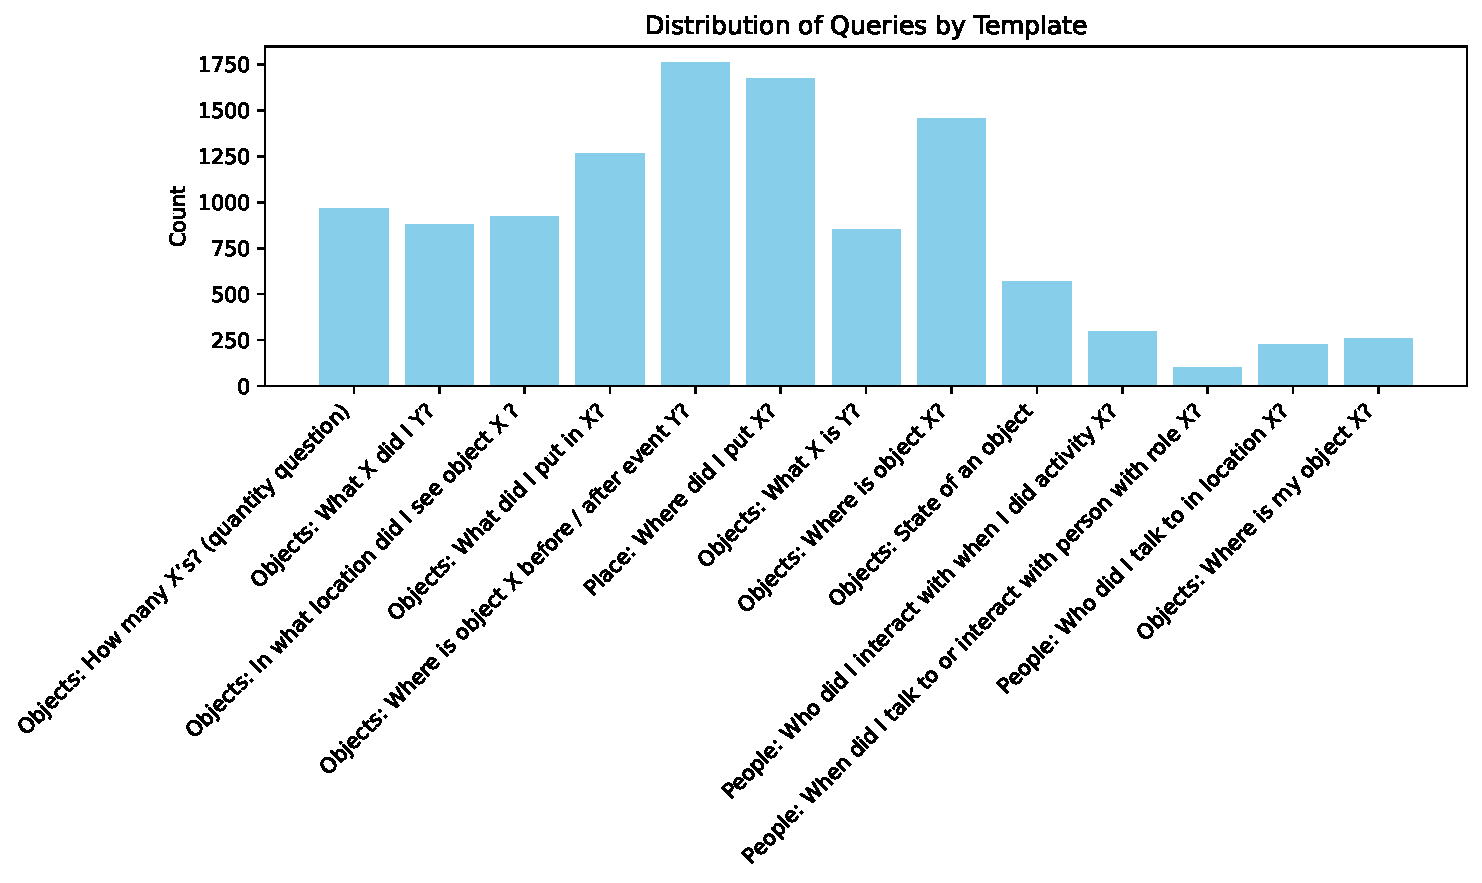
\includegraphics[width=0.48\textwidth]{Figure1.pdf} % adjust width as needed
\caption{Caption}
\label{fig:figure2}
\end{figure}

Analyzing the data retrieved through annotations yields valuable insights for our current task. Initially, we note that the average duration of clips is 522 seconds, with the majority lasting 480 seconds (8 minutes). Approximately 9.01\% of the dataset consists of short queries, defined as lasting four frames or less at a frame rate of 30 frames per second; these queries of approximately 0 seconds duration are excluded.

Another observation from plotting the distribution is the relative duration of each query compared to the total duration of its corresponding video clip. Notably, most queries encompass 2\% or less of the total clip duration. To support this finding, we analyzed the average response interval and found it to be 9.67 seconds.

In Figure 2 reported below, we illustrate the distribution of the number of queries per video, suggesting an average of 15 queries per video.

\begin{figure}[h]
\centering
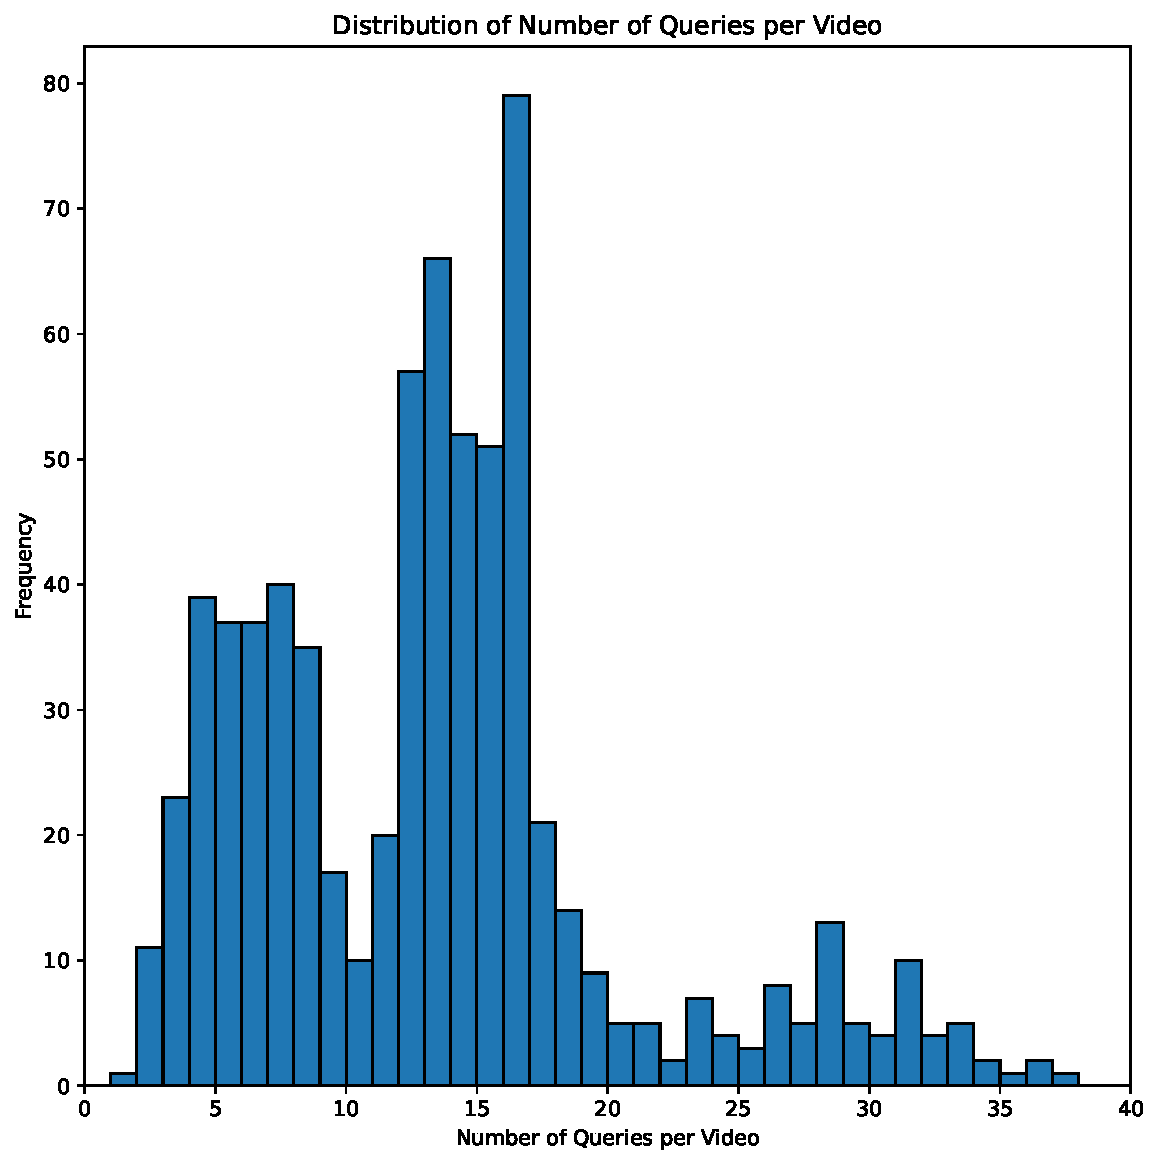
\includegraphics[width=0.3\textwidth]{Figure2.pdf} % adjust width as needed
\caption{Caption}
\label{fig:figure2}
\end{figure}

Finally, it's intriguing to note the correlation between each query and specific scenarios depicted in the video. Particularly, a significant number of queries (exceeding 100) are focused on the following scenarios: indoor navigation (walking), carpentry, cleaning/laundry, various jobs within construction and renovation companies (such as director of work, tiler, plumber, electrician, handyman, etc.), car mechanics, and cooking.


\section{Model architecture}
In this section, we delve into the architecture of the model, tracing its evolution from the first implementation to it subsequent enhancement through the integration of the QGH module and the transition to the BERT encoder, examining how these modifications contribute to the improved performance of the model.
VSLBase is the first implementation of our model for video span localization which leverages natural language queries to identify relevant segments within the video.
The model uses pre-extracted video features taken from pre-trained CNN (Convolutional Neural Network). To represent the query in an efficient way  Glove (Global vectors) embeddings are used,  so that the query itself is transformed into a dense vector. In the next step these word embeddings are fed to a bidirectional  LSTM network which outputs a context-aware representation of the query; these representations are then aligned through an attention mechanism to help the model focus on the relevant segments of the video(where most probably the answer to the query will be found).lastly, the output of the attention mechanism is used to predict the start and end times of the video segments that answer the given query. 
The model architecture comprises several key components: 
\begin{itemize}
 \item \textit{\textbf{Glove text encoder}}: Glove embeddings provide a dense  and fixed-size vector representation of the words in a high-dimensional space (going up to hundreds of dimensions) , capturing semantic similarities; words with similar meanings, or words that are used in similar contexts, have similar vector representations , which helps in understanding the context and semantics 
 \item \textit{\textbf{Pre-traine Convolutional Neural Network}}:the convolutional neural network is used to extract  high-level visual features from the video frames which are then encoded, typically in a sequence of frame-level embeddings  
 \item \textit{\textbf{Long Short-Term Memory network}}: both the video features and the textual features are fed into LSTM networks to capture the temporal dependencies in the video and the textual dependencies in the text; The Birectional LSTM (BiLSTM) processes the encoded sequences in both forward and backward directions, allowing the model to utilize information from both past and future contexts
 \item \textit{\textbf{Attention mechanism}}:: this mechanism aligns the encoded text and the query representation by computing attention scores that highlight relevant parts of the passage (video segment) to the query (it essentially calculates the relevance of each video frame to the given query) 
 
\end{itemize}

This initial implementation of VSLBase was significantly improved through two major enhancements: the integration of the QGH module and the BERT encoder. This enhancement model is known as VSLNet.
The Query-Guided Highlighting (QGH)  has been primarily introduced to better redefine the alignment between the query and the video segments; it essentially leverages additional context from the query to dynamically adjust the attention weights and highlights the video segments most relevant to the query. This mechanism results in more accurate predictions of the start and end times for the relevant video segments. On the other hand, the substitution of the Glove embeddings to the BERT (Bidirectional Encoder Representations from Transformers) encoder allows for a deeper understanding of the query and subsequently a more context-aware representation of it. So now, differently from the previous architecture, the model can understand the context of the query, rather than the individual words only.


\section{Proposed Approach}
\subsection{Task}
In the NLQ task, we use models that retrieve only the
information about the temporal interval of the video that
answers the input query, to return also a textual answer,
which could be more useful for the user, we need to use
Video Language Models(VLMs).\\
One problem of VLMs is that it is computationally expensive to process the entire video to answer the query. Therefore, we propose an approach that leverages the strengths of both type of models. We use a VslNet as first step of a pipeline to identify the short interval of interest. Then, we can cut the entire video to the interval of interest and feed it to a VLM alongside the query.
Another approach could be to aggregate the full video information to make it more feasible for the model. However, this could lead to a loss of detail.\\

The pipeline we used is shown in fig.\ref{fig:fullPipeline}, and for the VLM task, we chose Video-LLaVA.

\subsection{Video-LLava}
Video LLava is a Large Vision-Language model, so given a query and a visual input, its task is to produce a textual answer.  It is capable of simultaneously handling both image and videos. Many existing approaches encode images and videos into separate input spaces, but this can be a limitation. Instead, this model uses a unified visual representation for both modalities within the language feature space.\\
Also, in paper \cite{b8} it is shown that unified visual representation befits LLMs in learning both images and videos when compared to models specifically designed for one of the modalities.
\subsubsection{Model Structure}
The first step consists in extracting visual features (from videos or images). For this purpose, LanguageBind encoders are used \cite{b9}. These encoders can map different modalities into the textual feature space. At the end of this process, we obtain a unified visual representation.\\ 
The next step is to use a shared projection layer to project the features, then they are in the same space with the tokenized textual queries. We can then input all the data into a large LLM to get the answer.\\
A key point of Video LLaVA is the alignment of visual modalities before projection. LanguageBind naturally aligns image and language in shared feature space using pretrained encoders. To align video representation to the language space it uses 3 millions video-text pairs from VIDAL-10M\cite{b9}. Therefore, before projection, data from both modalities are in a unified feature space.

\begin{figure*}
  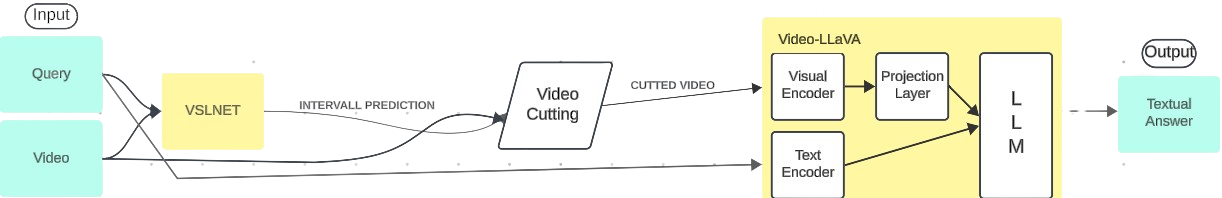
\includegraphics[width=\textwidth,height=4cm]{ProposedPipeLine-removebg-preview.png}
  \caption{Proposed Pipeline}
  \label{fig:fullPipeline}
\end{figure*}

\subsubsection{Training pipeline}
After obtaining the tokenized version of the textual input and visual signals input, the training consists in maximizing the likelyhood, so that the model can achieve multi-modal understanding capabilities.
This means that for each prediction in the training set, the objective is to maximize the probability of returning the ground-truth output based on the given input textual and visual tokens. \\
On of the strengths of the model is the simultaneous training on images and videos, with every batch containing both types of data.\\
In the first stage of training, the main focus is on associating the textual data with visual data using a extensive image/video-text pair dataset.\\
The second phase is the instruction tuning, the objective is still maximizing the likelihood but with the addition of a context variable. The context is the combination of the previous queries and answers.\\
Thus, at this stage, this model is trained to answer to more than one instruction. It must produce an output for several sequential and more complex queries, taking into consideration the entire conversation.
(Non mi sembra importante ma at this stage also the LLM are involved in training)

\subsection{Parameters}
During our tests we also observed the behaviour of the model bychanging some parameters related to output, the tested parameters were:
\\
\begin{itemize}
    \item \textit{\textbf{Max Length}}, it controls the lenght of the produced answer
    \item \textit{\textbf{Temperature}}, it controls the "creativity" of the answer, for high values, at each step, it flattens the probability distribution used to select the next word, so it can happen that the model selects also less probable words during the sequence generation, this could results in more creative but also less accurate answer
    \item \textit{\textbf{Top K}}, similarly to temperature, it also controls the diversity of the output, during the sequence generation, at each step, the model sample from the top K most probable textual tokens, higher value of K means higher diversity but also less accuracy
    \item \textit{\textbf{Top P}} in a different way from the previous, it controls the balance between accuracy and diversity, at each step, for the sampling are chosen the smallest number of tokens that have a cumulative probability greater or equal to P
     \item \textit{\textbf{Num Beam}} it controls the number of sequence that the model maintains at each step, an higher number can lead to more accurate solution. Basically at every iteration the algorithm try to combine to the current sequences with all the possible words, after doing that, the probability of all the new sequences is computed and the $Num Beam$ most probable sequences are kept for the following step
    
\end{itemize}

\section{Results}
\subsection{Numerical Results}
\subsubsection{NLQ task}
\hspace{1cm} \\
The metrics that we took into consideration to compare the obtained results are the following:
\begin{itemize}
    \item \textit{\textbf{IoU}}, Intersection over Union(IoU), it is the proportion between the intersection and the union of the ground-truth and predicted intervals\\
    \begin{equation}
        IoU = \frac{\text{PredictedInterval} \cap \text{Ground-TruthIntverval}}{\text{PredictedInterval} \cup \text{Ground-TruthIntverval}}
    \end{equation}
    \item \textit{\textbf{r@k}}, Recall at rank k (r@k) is used to measure how high the correct interval is positioned in the ranking of a prediction. %For example, r@1 indicates the percentage of predictions where the correct interval is ranked as the most probable solution.
    This metric is usefull because, for each query, multiple intervals are identified as possible solutions, and these intervals are ranked based on how well the model considers them to match the query
\end{itemize}

\begin{table}[h]
\centering
\caption{NLQ Performance}
\label{tab:performance}
\begin{tabular}{@{}lcccccc@{}}
\toprule
\multirow{2}{*}{Model} & \multirow{2}{*}{Features} & \multicolumn{2}{c}{IoU=0.3 (\%)} & \multicolumn{2}{c}{IoU=0.5 (\%)} \\ 
& & r@1  & r@5 & r@1   & r@5       \\ \midrule
VSLNet Paper Baseline & SlowFast & 5.45 & 10.74 & 3.12 & 6.63 \\ 
VSLNet & Omnivore & 6.48 & 14.04 & 3.72 & 8.70 \\ 
VSLNet & EgoVlp & 8.03 & 15.82 & 4.75 & 10.12 \\ 
VSLBase & Omnivore & 6.58 & 13.37 & 3.56 & 8.60 \\
VSLBase & EgoVlp & 7.18 & 14.74 & 4.26 & 9.65 \\
VSLNet* & Omnivore & 3.05 & 8.36 & 1.21 & 4.34 \\
VSLNet* & EgoVlp & 3.79 & 9.53 & 2.17 & 5.83 \\
\bottomrule
\end{tabular}
\captionsetup{font=footnotesize}
\caption*{VSLNet* is the version that uses GloVe as encoder instead of BERT.}
\end{table}
From the table, considering the cases in which the BERT encoder is used, we can notice that both VSLNet and VSLBase, using Omnivore and EgoVLP as pre-extracted features, perform better than VSLNet using SlowFast. It is important to specify that this improvement could also be due to the fact that annotations and features might have been updated since the publication of the original baseline in the paper.
\\
In particular, VSLNet with EgoVlp features significantly outperforms the others when we consider $IoU = 0.3$ and $r@1$, as well as when $IoU = 0.5$ and $r@5$.
\\
Models that do not use BERT as an encoder perform significantly worse than those that do. This could be because the BERT encoder is more sophisticated, indeed, it also takes into account the context in which words are used.







\subsubsection{Extension evaluation}
\hspace{1cm} \\
For the VLM task evaluation we decided to use the following metrics:
\begin{itemize}
    \item \textit{\textbf{R-F1}}, ROUGE-1 F1 Score(R-F1) is related to to overlap between the predicted sentence and the ground-truth. Computed as $F1-Score$ using the following precision and recall: 
    \begin{equation*}
        Precision = \frac{\text{\small Number of overlapping words}}{\text{ \small Total words in the prediction}}
    \end{equation*}
     \begin{equation}
        Recall = \frac{\text{\small Number of overlapping words}}{\text{\small Total words in the ground truth}}
    \end{equation}
    \item \textit{\textbf{METEOR}},The METEOR score is a more comprehensive metric than ROUGE. In addition to recall and precision, it incorporates an alignment component that measures how well the predictions align with the ground truth. Like ROUGE, METEOR produces a score between 0 and 1, however, precision and recall in METEOR are computed after an alignment process that includes stemming and synonyms matching
    \item \textit{\textbf{B-F1}}, The BERT F1 Score(B-F1) is as an advanced evaluation metric because it incorporates contextual understanding. It utilizes pre-trained contextual embeddings from BERT to compare the embeddings of the prediction sentence and ground truth sentence, measuring their similarity with cosine similarity. After this process it is possible to compute the recall, precision and F1 score(B-F1)
\end{itemize}

\begin{table}[h]
\centering
\caption{VLM Performance}
\label{tab:comparisonSCore}
\begin{tabular}{@{}lccc@{}}
\toprule
Configuration & R F1 & Meteor & B-F1 \\ \midrule
Default & 0.2789 & 0.2127 & 0.8667 \\
Temperature 2.0 & 0.0270 & 0.0219 & 0.8041 \\
Temperature 0.7 & 0.0528 & 0.0472 & 0.8113 \\
\bottomrule
\end{tabular}
\end{table}

In table \ref{tab:comparisonSCore} we show the score obtained, using models with some parameters variations.
The default parameters were:
\begin{itemize}[before=\footnotesize]
    \item $Temperature = 1.0$
    \item $Num Beam = 1$
    \item $Top K = 2$
    \item $Top P = 0.9$
    \item $Max new tokens = 100$
\end{itemize}
In the table, each configuration name represents the parameter we modified from the default settings to generate the new predictions and obtain the corresponding scores.
We have done multiple test on the parameter mentioned in \ref{Parameters}.Here we present the results obtained with the default parameters, the configuration that performed the worst, and the configuration that was closest to the default that performed the best.\\
It is notable that for both R-F1 and Meteor metrics, no configuration has achieved results as good as those obtained with the default parameters. This could be attributed to the fact that the ground truth used for reference was annotated by us, indicating that the default configuration produced predictions most similar to human language. When we examine the B-F1 scores, we see that they are generally higher and more consistent across different configurations, one explanation could be the BERT score's ability to assign high scores even when predictions and ground truths are quite dissimilar. A possible explanation, from our point of view, is that this could happen because B-F1 assesses similarity based on semantic similarity. Therefore, sentences can be considered similar if they contain words from the same semantic domain, regardless of exact phrasing.
\\
The previous consideration was more focused on the sentences semantic, if we talk about the accuracy of the predictions made by Video-LLaVA, the results is [mettere risultato]. To do this evaluation we had to manually chek if the answers was correct, since the scores values doesn't reflect the correctness. The total number of predictions was 50, we split them based on their category, and in [riferimento al grafico] it is possible to see the performance of the proposed approach among different categories.
As we studied the rates of success and failures of our model with the parameters set to their default values the meaningful results are the following: \\
\begin{itemize}[before=\footnotesize]
    \item overall, we have a 40% success rate,  with 20 correctly answered queries over a total of 50 queries
    \item for the Objects category we have a 36% success rate, with 15 correctly answered queries over a total of 42
    \item for the Place category we have a 67% success rate, with 4 correctly answered queries over a total of 6
    \item for the People category we have a 100% success rate, but on only 2 queries
   
\end{itemize}



\subsection{Qualitative Results}
In our study, visualizing the input video plays a crucial role in evaluating the model's ability to generate coherent answers. Below, we present some of the most intriguing qualitative results. These findings suggest that the model excels in scenarios requiring descriptive answers, offering insights that closely match manually annotated responses.

Notably, as illustrated in Figure X, the model successfully identified the object in question (broccoli) despite a short clip that did not provide a clear answer. This performance surpassed our observation, since we mistakenly identified the object as green peppers. By considering the entire video, it became evident that the correct identification was the one provided by the algorithm.

To further validate the model’s capability in accurately identifying answers, you can explore instances where the model correctly identifies the subjects of interest by visiting the following link: [LINK].

\begin{figure}[ht]
  \centering
  \animategraphics[autoplay,loop, height=4.5cm]{12}{53c86be4-190d-4410-8750-179a7edc70b3_}{001}{025}
  \caption{Prova}
  \label{fig:animation}
\end{figure}

However, the model exhibits limitations in specific tasks, particularly in counting objects or identifying precise quantities. Figure X exemplifies this: the model was asked to identify the number of fuse holders picked from a box. The model erroneously counted two fuse holders, whereas the ground truth indicated six. This discrepancy may be attributed to the fact that the individual in the video is holding only two fuse holders in their left hand at the end of the video, and the algorithm may struggle with maintaining an accurate understanding of the temporal sequence of actions.
The inaccuracy in counting extends to other queries, with additional examples available at the link mentioned above.

\begin{figure}[ht]
  \centering
  \animategraphics[autoplay,loop, height=4.5cm]{12}{53c86be4-190d-4410-8750-179a7edc70b3_}{001}{025}
  \caption{Prova}
  \label{fig:animation}
\end{figure}

Additionally, we observed that the model is often incorrect when answering yes/no questions. We highlight this issue in figure X, where the model provides a wrong answer despite the video being fairly clear. One assumption is that in these cases, when the model is forced to choose between two words for the first token, the probability to choose the wrong one is higher. This can be due to the binary choice limitation, where any slight bias can significantly impact the final decision. Moreover, the model's internal probability distribution for 'yes' and 'no' might be skewed, leading to systematic errors. Ambiguity in video interpretation and overfitting to training data, where certain answers are more frequent, could further contribute to this issue.

\begin{figure}[ht]
  \centering
  \animategraphics[autoplay,loop, height=4.5cm]{12}{53c86be4-190d-4410-8750-179a7edc70b3_}{001}{025}
  \caption{Prova}
  \label{fig:animation}
\end{figure}



\section*{References}

Please number citations consecutively within brackets \cite{b1}. The 
sentence punctuation follows the bracket \cite{b2}. Refer simply to the reference 
number, as in \cite{b3}---do not use ``Ref. \cite{b3}'' or ``reference \cite{b3}'' except at 
the beginning of a sentence: ``Reference \cite{b3} was the first $\ldots$''

Number footnotes separately in superscripts. Place the actual footnote at 
the bottom of the column in which it was cited. Do not put footnotes in the 
abstract or reference list. Use letters for table footnotes.

Unless there are six authors or more give all authors' names; do not use 
``et al.''. Papers that have not been published, even if they have been 
submitted for publication, should be cited as ``unpublished'' \cite{b4}. Papers 
that have been accepted for publication should be cited as ``in press'' \cite{b5}. 
Capitalize only the first word in a paper title, except for proper nouns and 
element symbols.

For papers published in translation journals, please give the English 
citation first, followed by the original foreign-language citation \cite{b6}.

\begin{thebibliography}{00}
\bibitem{b1} Santhosh Kumar Ramakrishnan and Ziad Al-Halah and Kristen Grauman, ``NaQ: Leveraging Narrations as Queries to Supervise Episodic Memory'', 2023.
\bibitem{b2} Jiyang Gao and Chen Sun and Zhenheng Yang and Ram Nevatia, ``TALL: Temporal Activity Localization via Language Query, '' 2017.
\bibitem{b3} Hao Zhang and Aixin Sun and Wei Jing and Joey Tianyi Zhou, ``Span-based Localizing Network for Natural Language Video Localization'' 2020.
\bibitem{b4} Chen, Jingyuan and Ma, Lin and Xinpeng, Chen and Jie, Zequn and Luo, Jiebo, ``Localizing Natural Language in Videos'' 2019.

\bibitem{b5} Lisa Anne Hendricks and Oliver Wang and Eli Shechtman and Josef Sivic and Trevor Darrell and Bryan Russell, ``Localizing Moments in Video with Temporal Language'' 2018.

\bibitem{b6} Deyao Zhu and Jun Chen and Xiaoqian Shen and Xiang Li and Mohamed Elhoseiny, ``MiniGPT-4: Enhancing Vision-Language Understanding with Advanced Large Language Models'' 2023.

\bibitem{b7} Qinghao Ye, Haiyang Xu, Guohai Xu, Jiabo Ye, Ming Yan, Yiyang Zhou, Junyang Wang, Anwen Hu, Pengcheng Shi, Yaya Shi, Chenliang Li, Yuanhong Xu, Hehong Chen, Junfeng Tian, Qi Qian, Ji Zhang, Fei Huang, Jingren Zhou, ``mPLUG-Owl: Modularization Empowers Large Language Models with Multimodality'' 2023.
\bibitem{b8} Lin, B., Zhu, B., Ye, Y., Ning, M., Jin, P., & Yuan, L. (2023). Video-llava: Learning united visual representation by alignment before projection. arXiv preprint arXiv:2311.10122.
\bibitem{b9}Bin Zhu, Bin Lin, Munan Ning, Yang Yan, Jiaxi Cui, HongFa Wang, Yatian Pang, Wenhao Jiang, Junwu Zhang, Zongwei Li, et al. Languagebind: Extending video-language pretrain- ing to n-modality by language-based semantic alignment. arXiv preprint arXiv:2310.01852, 2023.

\end{thebibliography}
\vspace{12pt}
\color{red}
IEEE conference templates contain guidance text for composing and formatting conference papers. Please ensure that all template text is removed from your conference paper prior to submission to the conference. Failure to remove the template text from your paper may result in your paper not being published.

\end{document}
